\documentclass[a4paper]{article}

\usepackage[utf8]{inputenc}
\usepackage[T2A]{fontenc}
\usepackage[russian]{babel}

\usepackage{mathtext}

\usepackage{listings}
\usepackage{color}

\definecolor{mygreen}{rgb}{0,0.6,0}
\definecolor{mygray}{rgb}{0.5,0.5,0.5}
\definecolor{mymauve}{rgb}{0.58,0,0.82}

\lstset{
	morekeywords={*,...}, % если хотите добавить ключевые слова
	keywordstyle=\color{blue},
	stringstyle=\color{mymauve},
	% Настройки отображения
	breaklines=true, % Перенос длинных строк
	basicstyle=\footnotesize, % Шрифт для отображения кода
	backgroundcolor=\color{white}, % Цвет фона кода
	frame=single,
	rulecolor=\color{black}, % Цвет рамки
	tabsize=3, % Размер табуляции в пробелах
	% Настройка отображения номеров строк. Если не нужно, то удалите весь блок
	numbers=left, % Слева отображаются номера строк
	stepnumber=1, % Каждую строку нумеровать
	numbersep=5pt, % Отступ от кода
	numberstyle=\tiny\color{mygray},
	% Для отображения русского языка
	extendedchars=true,
	literate={Ö}{{\"O}}1
	{Ä}{{\"A}}1
	{Ü}{{\"U}}1
	{ß}{{\ss}}1
	{ü}{{\"u}}1
	{ä}{{\"a}}1
	{ö}{{\"o}}1
	{~}{{\textasciitilde}}1
	{а}{{\selectfont\char224}}1
	{б}{{\selectfont\char225}}1
	{в}{{\selectfont\char226}}1
	{г}{{\selectfont\char227}}1
	{д}{{\selectfont\char228}}1
	{е}{{\selectfont\char229}}1
	{ё}{{\"e}}1
	{ж}{{\selectfont\char230}}1
	{з}{{\selectfont\char231}}1
	{и}{{\selectfont\char232}}1
	{й}{{\selectfont\char233}}1
	{к}{{\selectfont\char234}}1
	{л}{{\selectfont\char235}}1
	{м}{{\selectfont\char236}}1
	{н}{{\selectfont\char237}}1
	{о}{{\selectfont\char238}}1
	{п}{{\selectfont\char239}}1
	{р}{{\selectfont\char240}}1
	{с}{{\selectfont\char241}}1
	{т}{{\selectfont\char242}}1
	{у}{{\selectfont\char243}}1
	{ф}{{\selectfont\char244}}1
	{х}{{\selectfont\char245}}1
	{ц}{{\selectfont\char246}}1
	{ч}{{\selectfont\char247}}1
	{ш}{{\selectfont\char248}}1
	{щ}{{\selectfont\char249}}1
	{ъ}{{\selectfont\char250}}1
	{ы}{{\selectfont\char251}}1
	{ь}{{\selectfont\char252}}1
	{э}{{\selectfont\char253}}1
	{ю}{{\selectfont\char254}}1
	{я}{{\selectfont\char255}}1
	{А}{{\selectfont\char192}}1
	{Б}{{\selectfont\char193}}1
	{В}{{\selectfont\char194}}1
	{Г}{{\selectfont\char195}}1
	{Д}{{\selectfont\char196}}1
	{Е}{{\selectfont\char197}}1
	{Ё}{{\"E}}1
	{Ж}{{\selectfont\char198}}1
	{З}{{\selectfont\char199}}1
	{И}{{\selectfont\char200}}1
	{Й}{{\selectfont\char201}}1
	{К}{{\selectfont\char202}}1
	{Л}{{\selectfont\char203}}1
	{М}{{\selectfont\char204}}1
	{Н}{{\selectfont\char205}}1
	{О}{{\selectfont\char206}}1
	{П}{{\selectfont\char207}}1
	{Р}{{\selectfont\char208}}1
	{С}{{\selectfont\char209}}1
	{Т}{{\selectfont\char210}}1
	{У}{{\selectfont\char211}}1
	{Ф}{{\selectfont\char212}}1
	{Х}{{\selectfont\char213}}1
	{Ц}{{\selectfont\char214}}1
	{Ч}{{\selectfont\char215}}1
	{Ш}{{\selectfont\char216}}1
	{Щ}{{\selectfont\char217}}1
	{Ъ}{{\selectfont\char218}}1
	{Ы}{{\selectfont\char219}}1
	{Ь}{{\selectfont\char220}}1
	{Э}{{\selectfont\char221}}1
	{Ю}{{\selectfont\char222}}1
	{Я}{{\selectfont\char223}}1
	{і}{{\selectfont\char105}}1
	{ї}{{\selectfont\char168}}1
	{є}{{\selectfont\char185}}1
	{ґ}{{\selectfont\char160}}1
	{І}{{\selectfont\char73}}1
	{Ї}{{\selectfont\char136}}1
	{Є}{{\selectfont\char153}}1
	{Ґ}{{\selectfont\char128}}1
	{\{}{{{\color{black}\{}}}1 % Цвет скобок {
	{\}}{{{\color{black}\}}}}1 % Цвет скобок }
	,
%	title=\lstname
}

\usepackage{algorithmicx}
\usepackage{algpseudocode}

\usepackage{amssymb}
\usepackage{amsopn}
\usepackage{mathtools}

\usepackage{graphicx}

\usepackage[
a4paper, includefoot,
left=2cm, right=1cm, top=2cm, bottom=2cm,
]{geometry}

\usepackage[hidelinks]{hyperref}
\usepackage{multirow}
\usepackage{cmap}


\begin{document}

\begin{titlepage}

	\begin{center}

		\large Федеральное государственное автономное образовательное учреждение высшего образования \\
		\large «Санкт-Петербургский политехнический университет Петра Великого» \\
		\large Институт компьютерных наук и технологий \\
		\large Кафедра «Компьютерные интеллектуальные технологии» \\[4cm]

		\huge {\bf Курсовая работа} \\[0.5cm]
		\large {\bf Информационная система автомобилестроительного предприятия} \\[0.1cm]
		\large по дисциплине «Базы данных» \\[4cm]

	\end{center}

    \begin{center}
        \begin{minipage}[t]{4cm}
            \begin{flushleft}
                Выполнил студент гр. 23506/1
            \end{flushleft}
        \end{minipage}
        \hfill
        \begin{minipage}[t]{4cm}
            \begin{flushright}
            О.Д. Романов
            \end{flushright}
        \end{minipage} \\[0.5cm]

        \begin{minipage}[t]{4cm}
            \begin{flushleft}
                Руководитель старший преподаватель
            \end{flushleft}
            \flushleft
        \end{minipage}
        \hfill
        \begin{minipage}[t]{4cm}
            \begin{flushright}
                Н.В. Андреева
            \end{flushright}
        \end{minipage}
    \end{center}

    \begin{flushright}
        14 мая 2017
    \end{flushright}

	
	\vfill

	\begin{center}
	    \large Санкт-Петербург\\
	    \large \the\year
	\end{center}
 
\end{titlepage}

\section*{Задание на проектирование}

{\bf Срок сдачи законченной работы: } 22.05.2017

\underline{Начальное описание предметной области:}

Структурно предприятие состоит из цехов, которые в свою очередь подразделяются на участки.

Категории изделий, выпускаемых предприятием: грузовые, легковые автомобили, автобусы, сельскохозяйственные, дорожно-строительные машины, мотоциклы и прочие изделия.
Каждая категория изделий имеет специфические, присущие только ей атрибуты.
Например, для автобусов это вместимость, для сельскохозяйственных и дорожно-строительных машин - производительность и т.д.

По каждой категории изделий может собираться несколько видов изделий (под видом изделия понимается конкретная его разновидность / марка - например, автомобиль KIA Rio).
По конкретным экземплярам каждого вида ведётся журнал, где отмечаются даты завершения различных этапов жизненного цикла изделия: изготовление (сборка) / тестирование / передача дилеру / гарантийный ремонт.

Предприятие в основном состоит из производственных цехов, но также есть несколько вспомогательных (например, ремонтный, тестировочный).

Каждая категория изделий собирается в своём производственном цехе (в одном цехе может собираться несколько категорий изделий).
Цех структурно состоит из участков, на каждом из которых выполняется один вид работ: изготавливается определённая часть изделия (например, двигатель) либо производится сборка изделия в целом.
С каждой категорией изделия ассоциируется свой набор работ; другими словами, каждая категория в процессе изготовления должна пройти определённый набор участков в цехе.

Каждой категории инженерно-технического персонала (инженеры, технологи, техники) и рабочих (сборщики, токари, слесари, сварщики и пр.) также характерны атрибуты, свойственные только для этой группы.
Рабочие объединяются в бригады, которыми руководят бригадиры.
Бригадиры выбираются из числа рабочих.
Работу цеха возглавляет начальник цеха, а работу на участке - начальник участка, в подчинении которого находится несколько мастеров.
Каждый мастер координирует работу одной или нескольких бригад (но, в отличие от бригадира, не входит в состав конкретной бригады).
Мастера, начальники участков и цехов назначаются из числа инженерно-технического персонала.
Каждый начальник может руководить только одной структурной единицей (в т.ч. начальник одной структурной единицы не может быть в то же время начальником другой).

Работу по сборке конкретной категории изделия на определенном участке выполняет одна бригада рабочих, при этом она может обслуживать несколько участков / категорий и на одном участке может работать несколько бригад.

\begin{enumerate}

    \item Сотрудники могут быть либо рабочими, либо быть из инженерно-технического персонала (ИТП).
    \item Каждой категории инженерно-технического персонала характерны атрибуты, свойственные только для этой группы.
    \item Каждой категории рабочих характерны атрибуты, свойственные только для этой группы.
    \item В инженерно-технический персонал входят инженеры, технологи и техники.
    \item Рабочие объединяются в бригады.
    \item Бригадами руководят бригадиры.
    \item Бригадиры выбираются из числа рабочих.
    \item Мастера, начальники участков и цехов назначаются из числа инженерно-технического персонала.
    \item Работу цеха возглавляет начальник цеха.
    \item Работу на участке возглавляет начальник участка, в подчинении которого находится несколько мастеров.
    \item Работу по сборке конкретной категории изделия на определенном участке выполняет одна бригада рабочих, при этом она может обслуживать несколько участков / категорий и на одном участке может работать несколько бригад.
    \item Начальник цеха может руководить только одним цехом, а начальник участка может руководить только одним участком.
    \item Мастер может руководить бригадами на нескольких участках.
    \item Бригада может работать на нескольких участках.
    \item Цехи состоят из участков.
    \item Каждая категория в процессе изготовления должна пройти определённый набор участков в цехе.

    \item Представитель нженерно-технического персонала входит в какую-то категорию (инженеры, технологи, техники).
    \item Рабочий входит в какую-то категорию (сборщики, токари, слесари, сварщики и пр.).
    \item Цех структурно состоит из участков, на каждом из которых выполняется определенный вид работ: изготавливается определенная часть изделия или происходит сборка изделия целиком.
    \item Цех можеть быть либо производственным, либо вспомогательным.
    \item Каждая категория изделия собирается в своем производственном цехе.
    \item Каждая категория изделий имеет специфические, присущие только ей атрибуты.

    \item По каждой категории изделий может собираться несколько видов изделий.
    \item По конкретным экземплярам каждого вида ведётся журнал, где отмечаются даты завершения различных этапов жизненного цикла изделия.

\end{enumerate}

\underline{Варианты запросов к информационной системе:}
\begin{enumerate}

    \item Перечень видов изделий по категории, собираемой указанным цехом.
    В последней строке вывести общее число собираемых видов изделий.

    \item Количество экземпляров изделий каждого вида каждой категории, собранных предприятием за определенный отрезок времени.
    В последней строке вывести общее число собранных изделий.
    Примерный вид результата:

    \begin{tabular}{|p{6cm}|p{2cm}|p{1cm}|} \hline
        Категория & Вид & Кол-во \\ \hline
        Автобусы & АКБ-12 & 8 \\ \hline
        Автобусы & АКБ-05 & 0 \\ \hline
        Автомобили & ИЖ-400 & 12 \\ \hline
        ... & ... & ... \\ \hline
        Всего собрано (12.05.2010-18.07.2010): & & 48 \\ \hline
    \end{tabular}

    \item Данные о кадровом составе (ФИО, должность) по указанным категориям инженерно-технического персонала и рабочих;
    \item Число и перечень участков предприятия и их начальников (с указанием цехов).
    \item Перечень работ, которые проходит указанный вид изделия.
    \item Состав бригад, работающих на указанном участке указанного цеха: ФИО рабочего, номер бригады, номер участка, номер цеха. Отсортировать по номеру бригады.
    \item Перечень мастеров (ФИО) указанного участка указанного цеха и номера бригад, работы которых они координируют.
    \item Информация о цехах, в которых в настоящий момент собирается больше видов изделий, чем в среднем приходится на каждый производственный цех предприятия: номер цеха, название цеха, кол-во собираемых видов изделий, среднее количество видов изделий по цехам предприятия.
    \item Состав бригад, участвующих в сборке указанной категории изделия.
    \item ФИО и должности работников цеха, в котором собирается больше всего категорий изделий.

\end{enumerate}

{\bf Перечень подлежащих разработке вопросов:}
\begin{enumerate}
    \item Проанализировать предметную область, описание которой приведено в выданном варианте задания, и создать логическую модель базы данных.
    \item Провести нормализацию разработанной модели до 5НФ.
    \item Проверить разработанную модель средствами Data Model Validator.
    \item Устранить все замечания по модели, которые выявил Data Model Validator.
    \item Создать физическую модель базы данных, предусмотрев значения по умолчанию и условия проверки вводимых пользователем значений.
    \item Провести прямое проектирование – создать объекты базы данных в Oracle.
    \item Провести обратное проектирование базы данных из Oracle. Убедиться в том, что полученные в результате модели полностью аналогичны исходным.
    \item Проверить корректность произведённого прямого проектирования и выполнение требований, приведённых в описании предметной области (наличие ключей, значений по умолчанию, условий проверки вводимых пользователем значений, связей между таблицами и др.). Проверку произвести, внеся в таблицы базы данных минимум по 5 записей.
    \item Создать 10 SQL-запросов согласно выданному варианту задания. Проверить работоспособность написанных запросов.
    \item Добавить в физическую модель представление на основе SQL-запроса, выбранного по согласованию с преподавателем.
    \item Провести прямое проектирование (перенести созданное представление). Проверить работоспособность представления.
\end{enumerate}

\newpage
\tableofcontents
\newpage

\section{Введение}
В современном мире человек буквально на каждом шагу сталкивается с различными информационными системами.
Начиная от базы данных маленькой школы и заканчивая большими дата-центрами больших компаний.
Однако чем больше необходимо хранить информации, тем больше ее необходимо грамотно (нормализованно) хранить.
Система управления базами данных (СУБД) позволяет создать базу данных, хранить и обновлять в ней данные, а также
СУБД Oracle может быть использована в такой области деятельности, как автомобилестроительное предприятие.
Что я и покажу в данной курсовой работе.

Целью данной работы является спроектировать информационную систему автомобилестроительного предприятия, учитывая техническое задание.

Задачи, которые необходимо выполнить для достижения поставленной цели, перечислены в задании на проектирование.

\newpage

\section{Описание логической модели базы данных}

Диаграммы логической и физической моделей базы данных приведены в Приложении 1 и Приложении 2 соответственно.

\subsection{Сущности, их харрактеристики и связи}
В ходе анализа начального описания предметной области были выявлены следующие сущности:

\begin{enumerate}
    \item{Сотрудник}

    \begin{tabular}{|p{4cm}|p{3cm}|p{1cm}|p{1cm}|p{2cm}|} \hline

        {\bf COLUMN\_NAME} & {\bf DATA\_TYPE} & {\bf PK} & {\bf FK} & {\bf NULLABLE} \\ \hline
        Номер\_договора & NUMBER(6, 0) & YES & NO & NO \\ \hline
        Имя\_рабочего & VARCHAR2(12) & NO & NO & NO \\ \hline
        Фамилия\_рабочего & VARCHAR2(12) & NO & NO & NO \\ \hline
        Отчество\_рабочего & VARCHAR2(12) & NO & NO & YES \\ \hline

    \end{tabular}

    На предприятии работают сотрудики (в них входят рабочие и представители инженерно-технического персонала).

    \begin{tabular}{|p{4cm}|p{5cm}|} \hline

        {\bf COLUMN\_NAME} & {\bf Примечание} \\ \hline
        Номер\_договора &  Договор о найме на роботу, уникален для каждого работник \\ \hline
        Имя\_сотрудника &  Имя сотрудника \\ \hline
        Фамилия\_сотрудника & Фамилия сотрудника \\ \hline
        Отчество\_сотрудника & Отчество сотрудника, у человека может не быть фамилии \\ \hline

    \end{tabular}

    \item{ИТП}

    \begin{tabular}{|p{4cm}|p{3cm}|p{1cm}|p{1cm}|p{2cm}|} \hline

        {\bf COLUMN\_NAME} & {\bf DATA\_TYPE} & {\bf PK} & {\bf FK} & {\bf NULLABLE} \\ \hline
        Номер\_договора & NUMBER(6, 0) & YES & YES & NO \\ \hline
        ИД\_категории\_ИТП & NUMBER(2, 0) & NO & YES & NO \\ \hline

    \end{tabular}

    \underline{Сотрудник} может быть из \underline{инженерно-технического персонала} (1), что реализовано с помощью связи один-к-одному между соответствующими сущностями.

    \underline{Представитель инженерно-технического персонала} входит в какую-то \underline{категорию} (инженер, технолого и пр.), что реализовано с помощью связи один-ко-многим между соответствующими сущностями.

    \begin{tabular}{|p{4cm}|p{5cm}|} \hline

        {\bf COLUMN\_NAME} & {\bf Примечание} \\ \hline
        Номер\_договора & Договор о найме, уникален \\ \hline
        ИД\_категории\_ИТП & Категория представителя ИТП, у разных представителей может быть одинаковая категория \\ \hline

    \end{tabular}

    Ключевая группа XIE1ИТП:

    \begin{tabular}{|p{4cm}|p{5cm}|} \hline

        {\bf Имя атрибута} & {\bf Примечание} \\ \hline
        ИД\_категории\_ИТП & Индекс для FK \\ \hline

    \end{tabular}

    \item{Категория ИТП}

    \begin{tabular}{|p{4cm}|p{3cm}|p{1cm}|p{1cm}|p{2cm}|} \hline

        {\bf COLUMN\_NAME} & {\bf DATA\_TYPE} & {\bf PK} & {\bf FK} & {\bf NULLABLE} \\ \hline
        ИД\_категории\_ИТП & NUMBER(2, 0) & YES & NO & NO \\ \hline
        Название\_категории\_ИТП & VARCHAR2(15) & NO & NO & NO \\ \hline

    \end{tabular}

    Каждый представитель инженерно-технического персонала входит в какую-то категорию (17).

    \begin{tabular}{|p{4cm}|p{5cm}|} \hline

        {\bf COLUMN\_NAME} & {\bf Примечание} \\ \hline
        ИД\_категории\_ИТП &  Уникален \\ \hline
        Название\_категории\_ИТП & Название также уникально \\ \hline

    \end{tabular}

    Ключевая группа XAK1Категория\_ИТП:

    \begin{tabular}{|p{4cm}|p{5cm}|} \hline

        {\bf Имя атрибута} & {\bf Примечание} \\ \hline
        азвание\_категории\_ИТП & Альтернатива сурогатному ключу \\ \hline

    \end{tabular}

    \item{Атрибуты ИТП}

    \begin{tabular}{|p{4cm}|p{3cm}|p{1cm}|p{1cm}|p{2cm}|} \hline

        {\bf COLUMN\_NAME} & {\bf DATA\_TYPE} & {\bf PK} & {\bf FK} & {\bf NULLABLE} \\ \hline
        Название\_атрибута\_ИТП & VARCHAR2(15) & YES & NO & NO \\ \hline
        ИД\_категории\_ИТП & NUMBER(2, 0) & NO & YES & NO \\ \hline

    \end{tabular}

    Каждой \underline{категории инженерно-технического персонала} характерны \underline{атрибуты}, свойственные только для этой группы (2),
    что и реализовано с помощью связи один-ко-многим между соответствующими сущностями.

    \begin{tabular}{|p{4cm}|p{5cm}|} \hline

        {\bf COLUMN\_NAME} & {\bf Примечание} \\ \hline
        Название\_атрибута\_ИТП & Название атрибута, свойственного для какой-то категории ИТП. А так как атрибуты уникальный для каждой категории, то и название уникально \\ \hline
        ИД\_категории\_ИТП & Идентификатор категории, которой характерен этот атрибут \\ \hline

    \end{tabular}

    Ключевая группа XIE1Атрибуты\_ИТП:

    \begin{tabular}{|p{4cm}|p{5cm}|} \hline

        {\bf Имя атрибута} & {\bf Примечание} \\ \hline
        ИД\_категории\_ИТП & Индекс для FK \\ \hline

    \end{tabular}

    \item{Рабочий}

    \begin{tabular}{|p{4cm}|p{3cm}|p{1cm}|p{1cm}|p{2cm}|} \hline

        {\bf COLUMN\_NAME} & {\bf DATA\_TYPE} & {\bf PK} & {\bf FK} & {\bf NULLABLE} \\ \hline
        Номер\_договора & NUMBER(6, 0) & YES & YES & NO \\ \hline
        ИД\_категории\_рабочего & NUMBER(2, 0) & NO & YES & NO \\ \hline
        ИД\_бригады & NUMBER(5, 0) & NO & YES & NO \\ \hline

    \end{tabular}

    \underline{Сотрудник} может быть \underline{рабочим} (1), что реализовано с помощью связи один-к-одному между соответствующими сущностями.

    \underline{Рабочий} входит в какую-то \underline{категорию} (сборщики, токари и пр.), что реализовано с помощью связи один-ко-многим между соответствующими сущностями.

    \underline{Рабочие} объединяются в бригады (5), что реализовано с помощью связи один-ко-многим между соотвествующими сущностями.

    \begin{tabular}{|p{4cm}|p{5cm}|} \hline

        {\bf COLUMN\_NAME} & {\bf Примечание} \\ \hline
        Номер\_договора & Номер договора рабочего \\ \hline
        ИД\_категории\_рабочего & Категория, которой принадлежит рабочий \\ \hline
        ИД\_бригады & Бригада, в которой состоит рабочий \\ \hline

    \end{tabular}

    Ключевая группа XIE1Рабочий:

    \begin{tabular}{|p{4cm}|p{5cm}|} \hline

        {\bf Имя атрибута} & {\bf Примечание} \\ \hline
        ИД\_бригады & Индекс для FK \\ \hline

    \end{tabular}

    Ключевая группа XIE2Рабочий:

    \begin{tabular}{|p{4cm}|p{5cm}|} \hline

        {\bf Имя атрибута} & {\bf Примечание} \\ \hline
        ИД\_категории\_рабочего & Индекс для FK \\ \hline

    \end{tabular}

    \item{Категория рабочего}

    \begin{tabular}{|p{4cm}|p{3cm}|p{1cm}|p{1cm}|p{2cm}|} \hline

        {\bf COLUMN\_NAME} & {\bf DATA\_TYPE} & {\bf PK} & {\bf FK} & {\bf NULLABLE} \\ \hline
        ИД\_категории\_рабочего & NUMBER(2, 0) & YES & NO & NO \\ \hline
        Название\_категории\_рабочего & VARCHAR2(15) & NO & NO & NO \\ \hline

    \end{tabular}

    Каждый рабочий входит в какую-то категорию (18).

    \begin{tabular}{|p{4cm}|p{5cm}|} \hline

        {\bf COLUMN\_NAME} & {\bf Примечание} \\ \hline
        ИД\_категории\_рабочего & Идентификатор категории уникален \\ \hline
        Название\_категории\_рабочего & Название категории уникально \\ \hline

    \end{tabular}

    Ключевая группа XAK1Категория\_рабочего:

    \begin{tabular}{|p{4cm}|p{5cm}|} \hline

        {\bf Имя атрибута} & {\bf Примечание} \\ \hline
        Название\_категории\_рабочего & Альтернатива сурогатному ключу \\ \hline

    \end{tabular}

    \item{Атрибуты рабочего}

    \begin{tabular}{|p{4cm}|p{3cm}|p{1cm}|p{1cm}|p{2cm}|} \hline

        {\bf COLUMN\_NAME} & {\bf DATA\_TYPE} & {\bf PK} & {\bf FK} & {\bf NULLABLE} \\ \hline
        Название\_атрибута\_рабочего & VARCHAR2(15) & YES & NO & NO \\ \hline
        ИД\_категории\_рабочего & NUMBER(2, 0) & NO & YES & NO \\ \hline

    \end{tabular}

    Каждой \underline{категории рабочих} характерны \underline{атрибуты}, свойственные только для этой группы (3), что и реализовано с помощью связи одни-ко-многим между соответсвующими сущностями.

    \begin{tabular}{|p{4cm}|p{5cm}|} \hline

        {\bf COLUMN\_NAME} & {\bf Примечание} \\ \hline
        Название\_атрибута\_рабочего & Название уникально, так как атрибут свойственен только одной категории \\ \hline
        ИД\_категории\_рабочего & Идентификатор категории, для которой свойственен этот атрибут \\ \hline

    \end{tabular}

    Ключевая группа XIE1Атрибуты\_рабочего:

    \begin{tabular}{|p{4cm}|p{5cm}|} \hline

        {\bf Имя атрибута} & {\bf Примечание} \\ \hline
        ИД\_категории\_рабочего & Индекс для FK \\ \hline

    \end{tabular}

    \item{Бригада}

    \begin{tabular}{|p{4cm}|p{3cm}|p{1cm}|p{1cm}|p{2cm}|} \hline

        {\bf COLUMN\_NAME} & {\bf DATA\_TYPE} & {\bf PK} & {\bf FK} & {\bf NULLABLE} \\ \hline
        ИД\_бригады & NUMBER(5, 0) & YES & NO & NO \\ \hline
        Номер\_договора & NUMBER(6, 0) & NO & YES & NO \\ \hline

    \end{tabular}

    Бригадами руководят бригадиры (6).
    Бригадиры выбираются из числа рабочих (7).
    Реализуем связь один-ко-многим между соответствующими сущностями.

    \begin{tabular}{|p{4cm}|p{5cm}|} \hline

        {\bf COLUMN\_NAME} & {\bf Примечание} \\ \hline
        ИД\_бригады & Номер бригады \\ \hline
        Номер\_договора & Номер договора бригадира \\ \hline

    \end{tabular}

    Ключевая группа XIE1Бригада:

    \begin{tabular}{|p{4cm}|p{5cm}|} \hline

        {\bf Имя атрибута} & {\bf Примечание} \\ \hline
        Номер\_договора & Индекс для FK \\ \hline

    \end{tabular}

    \item{Мастер}

    \begin{tabular}{|p{4cm}|p{3cm}|p{1cm}|p{1cm}|p{2cm}|} \hline

        {\bf COLUMN\_NAME} & {\bf DATA\_TYPE} & {\bf PK} & {\bf FK} & {\bf NULLABLE} \\ \hline
        Номер\_договора & NUMBER(6, 0) & YES & YES & NO \\ \hline

    \end{tabular}

    \underline{Мастера} назначаются из \underline{инженерно-технического персонала} (8), что и реализовано связью один-к-одному.

    \begin{tabular}{|p{4cm}|p{5cm}|} \hline

        {\bf COLUMN\_NAME} & {\bf Примечание} \\ \hline
        Номер\_договора & Номер договора мастера \\ \hline

    \end{tabular}

    \item{Начальник участка}

    \begin{tabular}{|p{4cm}|p{3cm}|p{1cm}|p{1cm}|p{2cm}|} \hline

        {\bf COLUMN\_NAME} & {\bf DATA\_TYPE} & {\bf PK} & {\bf FK} & {\bf NULLABLE} \\ \hline
        Номер\_договора & NUMBER(6, 0) & YES & YES & NO \\ \hline

    \end{tabular}

    \underline{Начальники участка} назначаются из \underline{инженерно-технического персонала} (8), что и реализовано связью один-к-одному.

    \begin{tabular}{|p{4cm}|p{5cm}|} \hline

        {\bf COLUMN\_NAME} & {\bf Примечание} \\ \hline
        Номер\_договора & Номер договора начальника участка \\ \hline

    \end{tabular}

    \item{Начальник цеха}

    \begin{tabular}{|p{4cm}|p{3cm}|p{1cm}|p{1cm}|p{2cm}|} \hline

        {\bf COLUMN\_NAME} & {\bf DATA\_TYPE} & {\bf PK} & {\bf FK} & {\bf NULLABLE} \\ \hline
        Номер\_договора & NUMBER(6, 0) & YES & YES & NO \\ \hline

    \end{tabular}

    \underline{Начальники цеха} назначаются из \underline{инженерно-технического персонала} (8), что и реализовано связью один-к-одному.

    \begin{tabular}{|p{4cm}|p{5cm}|} \hline

        {\bf COLUMN\_NAME} & {\bf Примечание} \\ \hline
        Номер\_договора & Номер договора начальника цеха \\ \hline

    \end{tabular}

    \item Мастер\_начальник

    \begin{tabular}{|p{4cm}|p{3cm}|p{1cm}|p{1cm}|p{2cm}|} \hline

        {\bf COLUMN\_NAME} & {\bf DATA\_TYPE} & {\bf PK} & {\bf FK} & {\bf NULLABLE} \\ \hline
        Договор\_мастер & NUMBER(6, 0) & YES & YES & NO \\ \hline
        Договор\_нач\_уч & NUMBER(6, 0) & YES & YES & NO \\ \hline

    \end{tabular}

    В подчинении \underline{начальника участка} находятся несколько \underline{мастеров} (10) и у мастера может быть несколько начальников (13).
    Что реализовывается связью один-ко-многим между соответствующими сущностями.

    \begin{tabular}{|p{4cm}|p{5cm}|} \hline

        {\bf COLUMN\_NAME} & {\bf Примечание} \\ \hline
        Договор\_мастер & Договор мастера, который находится в подченении начальника участка \\ \hline
        Договор\_нач\_уч & Договор начальника участка, в подченении которого находится мастер \\ \hline

    \end{tabular}

    Ключевая группа XIE1Мастер\_начальник:

    \begin{tabular}{|p{4cm}|p{5cm}|} \hline

        {\bf Имя атрибута} & {\bf Примечание} \\ \hline
        Договор\_нач\_уч & Индекс для FK \\ \hline

    \end{tabular}

    \item Мастер\_бригада

    \begin{tabular}{|p{4cm}|p{3cm}|p{1cm}|p{1cm}|p{2cm}|} \hline

        {\bf COLUMN\_NAME} & {\bf DATA\_TYPE} & {\bf PK} & {\bf FK} & {\bf NULLABLE} \\ \hline
        ИД\_бригады & NUMBER(5, 0) & YES & YES & NO \\ \hline
        Договор\_мастера & NUMBER(6, 0) & YES & YES & NO \\ \hline

    \end{tabular}

    Одна бригада может обслуживать несколько участков (11), а следовательно \underline{бригадой} могут руководить несколько \underline{мастеров}.
    По сути, данная таблица разрешает связь многие-ко-многим.

    \begin{tabular}{|p{4cm}|p{5cm}|} \hline

        {\bf COLUMN\_NAME} & {\bf Примечание} \\ \hline
        ИД\_бригады & Номер бригады, которой руководит мастер \\ \hline
        Договор\_мастера & Номер договора мастера, который руководит брмгадой \\ \hline

    \end{tabular}

    Ключевая группа XIE1Мастер\_бригада:

    \begin{tabular}{|p{4cm}|p{5cm}|} \hline

        {\bf Имя атрибута} & {\bf Примечание} \\ \hline
        Номер\_договора & Индекс для FK \\ \hline

    \end{tabular}

    \item{Участок}

    \begin{tabular}{|p{4cm}|p{3cm}|p{1cm}|p{1cm}|p{2cm}|} \hline

        {\bf COLUMN\_NAME} & {\bf DATA\_TYPE} & {\bf PK} & {\bf FK} & {\bf NULLABLE} \\ \hline
        Номер\_участка & NUMBER(3, 0) & YES & NO & NO \\ \hline
        Номер\_цеха & NUMBER(3, 0) & YES & YES & NO \\ \hline
        Тип\_участка & VARCHAR2(9) & NO & NO & NO \\ \hline
        Номер\_договора & NUMBER(6, 0) & NO & YES & NO \\ \hline

    \end{tabular}

    У \underline{участка} есть \underline{начальник участка} (10), что и реализовано с помощью связи один-к-одному между соответсвующими сущностями.
    \underline{Участок} находится в каком-то одном \underline{цеху} (15), что и реализовано с помощью связи многие-к-одному между соответсвующими сущностями.

    \begin{tabular}{|p{4cm}|p{5cm}|} \hline

        {\bf COLUMN\_NAME} & {\bf Примечание} \\ \hline
        Номер\_участка & Уникален в пределах цеха \\ \hline
        Номер\_цеха & Уникален в пределах предприятия \\ \hline
        Тип\_участка &  На участке может либо изготавливаться изделие, либо происходить сборка целиком (19) \\ \hline
        Номер\_договора & Номер договора начальника участка \\ \hline

    \end{tabular}

    Ключевая группа XIE3Участок:

    \begin{tabular}{|p{4cm}|p{5cm}|} \hline

        {\bf Имя атрибута} & {\bf Примечание} \\ \hline
        Номер\_договора & Индекс для FK \\ \hline

    \end{tabular}

    Ключевая группа XIE2Участок:

    \begin{tabular}{|p{4cm}|p{5cm}|} \hline

        {\bf Имя атрибута} & {\bf Примечание} \\ \hline
        Номер\_цеха & Индекс для FK \\ \hline

    \end{tabular}

    \item{Цех}

    \begin{tabular}{|p{4cm}|p{3cm}|p{1cm}|p{1cm}|p{2cm}|} \hline

        {\bf COLUMN\_NAME} & {\bf DATA\_TYPE} & {\bf PK} & {\bf FK} & {\bf NULLABLE} \\ \hline
        Номер\_цеха & NUMBER(3, 0) & YES & NO & NO \\ \hline
        Номер\_договора & NUMBER(6, 0) & NO & YES & NO \\ \hline

    \end{tabular}

    \underline{Цехом} руководит \underline{начальник цеха} (9), что и реализовано с помощью связи один-к-одному между соответсвующими сущностями.

    \begin{tabular}{|p{4cm}|p{5cm}|} \hline

        {\bf COLUMN\_NAME} & {\bf Примечание} \\ \hline
        Номер\_цеха & Уникален в пределах предприятия \\ \hline
        Номер\_договора & Номер договора начальника цеха \\ \hline

    \end{tabular}

    Ключевая группа XIE1Цех:

    \begin{tabular}{|p{4cm}|p{5cm}|} \hline

        {\bf Имя атрибута} & {\bf Примечание} \\ \hline
        Номер\_договора & Индекс для FK \\ \hline

    \end{tabular}

    \item{Вспомогат\_цех}

    \begin{tabular}{|p{4cm}|p{3cm}|p{1cm}|p{1cm}|p{2cm}|} \hline

        {\bf COLUMN\_NAME} & {\bf DATA\_TYPE} & {\bf PK} & {\bf FK} & {\bf NULLABLE} \\ \hline
        Номер\_цеха & NUMBER(3, 0) & YES & YES & NO \\ \hline

    \end{tabular}

   \underline{Цех} может быть \underline{вспомогательным} (20), что и реализовано с помощью связи один-к-одному между соответствующими сущностями.

    Обосную, почему нужно использовать категориальную связь (логический уровень) в данном случае.
    Цех может быть двух типов.
    Можно было бы просто добавить атрибут, у которого было бы ограничение на одпустимые значения (например, VARCHAR2 и значения "производственный" и "вспомогательный").
    Однако по условию, каждая категория изделия собирается в своем производственном цехе(21).
    Именно для отличия типов цехов и было решено сделать такое решение.

    \begin{tabular}{|p{4cm}|p{5cm}|} \hline

        {\bf COLUMN\_NAME} & {\bf Примечание} \\ \hline
        Номер\_цеха & Уникален в пределах предприятия \\ \hline

    \end{tabular}

    \item{Производств\_цех}

    \begin{tabular}{|p{4cm}|p{3cm}|p{1cm}|p{1cm}|p{2cm}|} \hline

        {\bf COLUMN\_NAME} & {\bf DATA\_TYPE} & {\bf PK} & {\bf FK} & {\bf NULLABLE} \\ \hline
        Номер\_цеха & NUMBER(3, 0) & YES & YES & NO \\ \hline

    \end{tabular}

   \underline{Цех} может быть \underline{производственным} (20), что и реализовано с помощью связи один-к-одному между соответствующими сущностями.

    \begin{tabular}{|p{4cm}|p{5cm}|} \hline

        {\bf COLUMN\_NAME} & {\bf Примечание} \\ \hline
        Номер\_цеха & Уникален в пределах предприятия \\ \hline

    \end{tabular}

    \item{Журнал}

    \begin{tabular}{|p{4cm}|p{3cm}|p{1cm}|p{1cm}|p{2cm}|} \hline

        {\bf COLUMN\_NAME} & {\bf DATA\_TYPE} & {\bf PK} & {\bf FK} & {\bf NULLABLE} \\ \hline
        Позиция\_в\_журнале & NUMBER(7, 0) & YES & NO & NO \\ \hline
        Название\_вида\_изделия & VARCHAR2(15) & NO & YES & NO \\ \hline
        Начало & DATE & NO & NO & NO \\ \hline
        Завершение & DATE & NO & NO & YES \\ \hline
        Номер\_участка & NUMBER(3, 0) & NO & NO & NO \\ \hline

    \end{tabular}

    По конкретным \underline{экземплярам} ведётся \underline{журнал}, где отмечаются даты завершения различных этапов жизненного цикла изделия (24), что и реализовано с помощью связи один-ко-многим между соответсвующими сущностями.

    Обосную, почему нельзя реализовать связь многие-ко-многим между \underline{работами} и \underline{журналом}.
    Казалось бы, это позволит создать правильное ограничение на добавление корректного участка в журнале.

    Разрешим связь многие-ко-многим с помощью ассоциативной таблицы.
    Назовем её R.
    Для того, чтобы проверять равенство участков в R мы можем просто добавить ограничение.
    Для этого вынесем в ПК \underline{журнала} Название\_вида\_изделия, Начало, Номер\_участка.

    Получится, что в R будет следующий первичный ключ: Название\_вида\_изделия, Начало, Номер\_участка1 (из Журнал), Название\_категории\_изделия, Номер\_участка2 (Из R).
    Можно выставить ограничение на равенство Номер\_участка1 и Номер\_участка2 (это хорошо).

    Однако Название\_вида\_изделия функционально зависит от Название\_категории\_изделия.
    К тому же можно будет добавить вид изделия, который не принадлежит своей категории изделия, что недопустимо.

    Полагаю, что эту ситауцию можно решить с использованием триггеров.
    Однако как мне кажется, это плохой способ, так как это приведет как минимум к падению производительности.
    К тому же ими было запрещено пользоваться.

    Ключевая группа XIE1Журнал:

    \begin{tabular}{|p{4cm}|p{5cm}|} \hline

        {\bf Имя атрибута} & {\bf Примечание} \\ \hline
        Название\_вида\_изделия & Индекс для FK \\ \hline

    \end{tabular}

    \item{Вид изделия}

    \begin{tabular}{|p{4cm}|p{3cm}|p{1cm}|p{1cm}|p{2cm}|} \hline

        {\bf COLUMN\_NAME} & {\bf DATA\_TYPE} & {\bf PK} & {\bf FK} & {\bf NULLABLE} \\ \hline
        Название\_вида\_изделия & VARCHAR2(15) & YES & NO & NO \\ \hline
        Название\_категории\_изделия & VARCHAR2(15) & NO & YES & NO \\ \hline

    \end{tabular}

    По каждой \underline{категории изделий} может собираться несколько \underline{видов изделий} (23), что и реализовано связью один-ко-многим между соответсвующими сущностями.

    \begin{tabular}{|p{4cm}|p{5cm}|} \hline

        {\bf COLUMN\_NAME} & {\bf Примечание} \\ \hline
        Название\_вида\_изделия & Уникально. Полагаем, что в название войдет полное имя. Например, мотоцикл BMW и автомобиль BMW будут иметь полные имена (т.е. BMW R75 и BMW X5).  \\ \hline
        Название\_категории\_изделия & Уникально, у разных видов может быть одна категория \\ \hline

    \end{tabular}

    Ключевая группа XIE1Вид\_изделия:

    \begin{tabular}{|p{4cm}|p{5cm}|} \hline

        {\bf Имя атрибута} & {\bf Примечание} \\ \hline
        Название\_категории\_изделия & Индекс для FK \\ \hline

    \end{tabular}

    \item{Категория изделия}

    \begin{tabular}{|p{4cm}|p{3cm}|p{1cm}|p{1cm}|p{2cm}|} \hline

        {\bf COLUMN\_NAME} & {\bf DATA\_TYPE} & {\bf PK} & {\bf FK} & {\bf NULLABLE} \\ \hline
        Название\_категории\_изделия & VARCHAR2(15) & YES & NO & NO \\ \hline
        Номер\_цеха & NUMBER(3, 0) & NO & YES & NO \\ \hline

    \end{tabular}

    Каждая \underline{категория изделия} собирается в своем \underline{производственном цехе} (21), что и реализовано с помощью связи многие-к-одному.

    \begin{tabular}{|p{4cm}|p{5cm}|} \hline

        {\bf COLUMN\_NAME} & {\bf Примечание} \\ \hline
        Название\_категории\_изделия & Название категории изделия уникально \\ \hline
        Номер\_цеха & Номер вспомогательного цеха, в котором собирается данное изделие. В одном вспомогательном цехе может собираться несколько категорий изделий. Не уникален \\ \hline

    \end{tabular}

    Ключевая группа XIE1Категория\_изделия:

    \begin{tabular}{|p{4cm}|p{5cm}|} \hline

        {\bf Имя атрибута} & {\bf Примечание} \\ \hline
        Номер\_цеха & Индекс для FK \\ \hline

    \end{tabular}

    \item{Атрибуты изделия}

    \begin{tabular}{|p{4cm}|p{3cm}|p{1cm}|p{1cm}|p{2cm}|} \hline

        {\bf COLUMN\_NAME} & {\bf DATA\_TYPE} & {\bf PK} & {\bf FK} & {\bf NULLABLE} \\ \hline
        Название\_атрибута\_изделия & VARCHAR2(15) & YES & NO & NO \\ \hline
        Название\_категории\_изделия & VARCHAR2(15) & NO & YES & NO \\ \hline

    \end{tabular}

    Каждая \underline{категория изделий} имеет специфические, присущие только ей \underline{атрибуты} (22), что и реализовано с помощью связи один-ко-многим между соотвествующими сущностями.

    \begin{tabular}{|p{4cm}|p{5cm}|} \hline

        {\bf COLUMN\_NAME} & {\bf Примечание} \\ \hline
        Название\_атрибута\_изделия & Атрибут уникален \\ \hline
        Название\_категории\_изделия & Название категории, которой присущ этот атрибут \\ \hline

    \end{tabular}

    Ключевая группа XIE1Атрибуты\_изделия:

    \begin{tabular}{|p{4cm}|p{5cm}|} \hline

        {\bf Имя атрибута} & {\bf Примечание} \\ \hline
        Название\_категории\_изделия & Индекс для FK \\ \hline

    \end{tabular}

    \item Работы

    \begin{tabular}{|p{4cm}|p{3cm}|p{1cm}|p{1cm}|p{2cm}|} \hline

        {\bf COLUMN\_NAME} & {\bf DATA\_TYPE} & {\bf PK} & {\bf FK} & {\bf NULLABLE} \\ \hline
        Название\_категории\_изделия & VARCHAR2(15) & YES & YES & NO \\ \hline
        Номер\_участка & NUMBER(3, 0) & YES & NO & NO \\ \hline

    \end{tabular}

    Каждая \underline{категория изделий} должна пройти определенный набор \underline{участков} в цехе (16).

    В данном случае мы не можем реализовать эту идею с помощью связи многие-ко-многим между соответствующими таблицами.
    Так как у нас появится ассоциативная таблица, назовем её R.
    У R будет следующий первичный ключ: Номер\_участка, Номер\_цеха и Название\_категории\_изделия.

    Во-первых, Номер\_цеха функционально зависит от Название\_категории\_изделия.

    Во-вторых, мы по прежнему не сможем проверять на согласованность номеров цеха.
    Чтобы можно было проверять на равенство в отношении R, нам надо будет добавить Номер\_цеха в PK отношения Категория\_изделия.
    Что в свою очередь скажется на ошибке нормализации:
    Номер\_цеха функционально зависит от Название\_категории\_изделия в отношении Категория\_изделия.

    Полагаю, что эту ситауцию можно решить с использованием триггеров.
    Однако как мне кажется, это плохой способ, так как это приведет как минимум к падению производительности.
    К тому же ими было запрещено пользоваться.

    \begin{tabular}{|p{4cm}|p{5cm}|} \hline

        {\bf COLUMN\_NAME} & {\bf Примечание} \\ \hline
        Название\_категории\_изделия & Название категории изделия\\ \hline
        Номер\_участка & Номер участка, в котором должна пройти сборка \\ \hline

    \end{tabular}

    Ключевая группа XIE1Работы:

    \begin{tabular}{|p{4cm}|p{5cm}|} \hline

        {\bf Имя атрибута} & {\bf Примечание} \\ \hline
        Название\_категории\_изделия & Индекс для FK \\ \hline

    \end{tabular}

\end{enumerate}

\subsection {Нормализация}
Нормализацией называется формальная процедура, в ходе которой создается оптимизированная структура базы данных, позволяющая избегать различные виды аномалий.

\begin{itemize}
    \item Первая нормальная форма (1 НФ)
    \item Вторая нормальная форма (2 НФ)
    \item Третья нормальная форма (3 НФ)
    \item Нормальная форма Бойса-Кодда (НФБК)
    \item Четвертая нормальная форма (4 НФ)
    \item Пятая нормальная форма (5 НФ)
\end{itemize}

{\bf Проверим на первую нормальную форму:}

Отношение находится в первой нормальной форме, тогда, когда на пересечении каждой строки и каждого столбца содержится ровно одно значение.
Во всех приведенных сущностях соблюдается атомарность данных.
Следовательно, все отношения в модели подчиняются 1 НФ.

{\bf Проверим на 2 нормальную форму:}

Отношение находится во второй нормальной форме тогда, когда отношение находится в 1 НФ, и нет неключевых атрибутов, зависящих от части сложного ключа.
Проверять нужно только сущности, содержащие больше одного ключевого атрибута:

\begin{itemize}

    \item Мастер\_бригада({\bf Номер\_договора}, {\bf ИД\_бригады})
    \item Мастер\_начальник({\bf Договор\_нач\_уч}, {\bf Договор\_мастер})
    \item Участок({\bf Номер\_участка}, {\bf Номер\_цеха}, Тип\_участка, Номер\_договора)
    \item Работы({\bf Название\_категории\_изделия}, {\bf Номер\_участка})

\end{itemize}

У сущностей Мастер\_бригада, Мастер\_начальник и Работы нет неключевых атрибутов.
У сущности Участок:
\begin{itemize}

    \item Тип\_участка не зависит от номера участка, так как это могут быть участки из разных цехов.
    Тип\_участка не зависит от номера цеха, так как это могут быть цеха с разными участками.
    \item Номер\_договора не зависит от номера участка, так как это могут быть участки из разных цехов.
    Номер\_договора не зависит от номера цеха, так как это могут быть цеха с разными участками.

\end{itemize}

Следовательно, все отношения в модели находятся в 2 НФ.

{\bf Проверим на 3 нормальную форму:}

Отношение находится в третьей нормальной форме тогда, когда отношение находится в 2НФ, и все неключевые атрибуты взаимно независимы.
Проверять нужно только сущности, содержащие больше одного неключевого атрибута:

\begin{itemize}

    \item Сотрудник({\bf Номер\_договора}, Имя\_сотрудника, Фамилия\_сотрудника, Отчество\_сотрудника)
    \item Рабочий({\bf Номер\_договора}, ИД\_категории\_рабочего, ИД\_бригады)
    \item Участок({\bf Номер\_участка}, {\bf Номер\_цеха}, Тип\_участка, Номер\_договора)
    \item Журнал({\bf Позиция\_в\_журнале}, Начало, Завершение, Название\_вида\_изделия, Номер\_участка)
\end{itemize}

Рассмотрим эти сущности:

\begin{itemize}
    \item В сущности \underline{сотрудник} фамилия не зависит от имени или отчества, имя не зависит от фамилии или отчетства, а также отчетсво не зависит от имени или фамилии.

    \item В сущности \underline{рабочий} катеория рабочего не зависит от номера его бригады, также как и бригада не зависит от его категории.

    \item В сущности \underline{участок} номер договора начальника не зависит от типа участка, точно также как и тип участка не зависит от начальника участка.

    \item В сущности \underline{журнал} номер участка не зависит от даты завершения работы, а дата завершения работы не завист от номера участка.

\end{itemize}

Следовательно, все отношения в модели находятся в 3 НФ.

{\bf Проверка на нормальную форму Бойса-Кодда:}

Отношение находится в нормальной форме Бойса-Кодда тогда, когда отношение находится в 3 НФ, и любая выполняемая для этого отношения нетривиальная и минимальная функциональная зависимость имеет в качестве детерминанта некоторый возможный ключ данного отношения.
Проверять нужно только сущности, содержащие несколько пересекающихся потенциальных ключей: таких сущностей нет.

Следовательно, все модели в сущности находятся в НФБК.

{\bf Проверка на 4 нормальную форму:}

Отношение находится в четвертой нормальной форме тогда, когда отношение находится в НФБК и не содержит нетривиальных многозначных зависимостей.
Проверять нужно только сущности, имеющие в составе первичного ключа три атрибута и более: таких сущностей нет.

Следовательно, все модели в сущности находятся в 4 НФ.

{\bf Проверка на 5 нормальную форму:}

Отношение находится в пятой нормальной форме тогда, когда отношение находится в 4 НФ, и каждая нетривиальная зависимость соединения в нём определяется потенциальным ключом (ключами) этого отношения.
Проверять нужно только сущности, имеющие в составе первичного ключа три атрибута и более: таких сущностей нет.

Следовательно, все модели в сущности находятся в 5 НФ.

\subsection{Условия проверки и значения по умолчанию для атрибутов}

Для атрибута {\bf Тип\_участка} сущности \underline{Участок} были определены допустимые значения: Изготовка" и "Сборка".
Так как на участке может выполняться один из этих видов работ (19).

\section {Отчёт по замечаниям ERwin Data Model Validator}

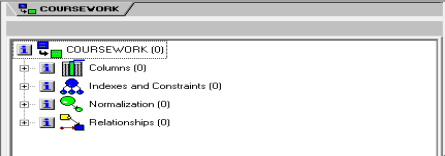
\includegraphics[width=12cm]{./screenshots/validator/validator.png}

ERwin Data Model Validator выдает ошибку Infinite Loop.
Это связано с тем, что отношения Бригада и Рабочий имеют две связи один ко многим.
Так как по условию нам дано следующее: рабочие объединяются в бригады, которыми руководят бригадиры, а бригадиры выбираются из числа рабочих.
Следовательно, выбранные связи обоснованы.

Обосную, почему эта ошибка не окажет никакого воздействия не схему.
Связи имеют Cardinality: Zero, One or More.
А следовательно, даже при пустой таблице мы можем вставить данные, указав Null.

Использование No Action on delete поможет нам запретить удаление бригады, пока мы не перевели всех ее работников.
Да и неприйтной ситуации с Delete Cascade можно избежать

\section{Реализация запросов к базе данных}

\begin{enumerate}

    \item Перечень видов изделий по категории, собираемой указанным цехом.
    В последней строке вывести общее число собираемых видов изделий.

    \lstinputlisting[language=SQL]{../sources/queries/task1.sql}

    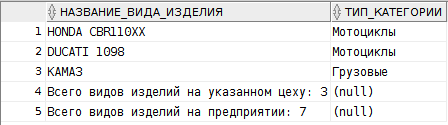
\includegraphics[width=11cm]{./screenshots/results/result1.png}

    \item Количество экземпляров изделий каждого вида каждой категории, собранных предприятием за определенный отрезок времени.
    В последней строке вывести общее число собранных изделий.

    \lstinputlisting[language=SQL]{../sources/queries/task2.sql}

    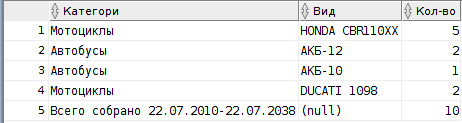
\includegraphics[width=11cm]{./screenshots/results/result2.png}

    \item Данные о кадровом составе (ФИО, должность) по указанным категориям инженерно-технического персонала и рабочих;

    \lstinputlisting[language=SQL]{../sources/queries/task3.sql}

    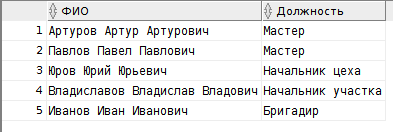
\includegraphics[width=11cm]{./screenshots/results/result3.png}

    \item Число и перечень участков предприятия и их начальников (с указанием цехов).

    \lstinputlisting[language=SQL]{../sources/queries/task4.sql}

    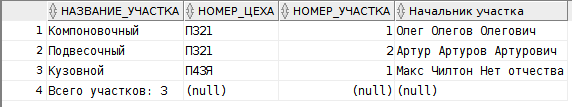
\includegraphics[width=11cm]{./screenshots/results/result4.png}

    \item Перечень работ, которые проходит указанный вид изделия.

    \lstinputlisting[language=SQL]{../sources/queries/task5.sql}

    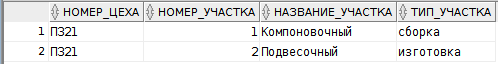
\includegraphics[width=11cm]{./screenshots/results/result5.png}

    \item Состав бригад, работающих на указанном участке указанного цеха: ФИО рабочего, номер бригады, номер участка, номер цеха. Отсортировать по номеру бригады.

    \lstinputlisting[language=SQL]{../sources/queries/task6.sql}

    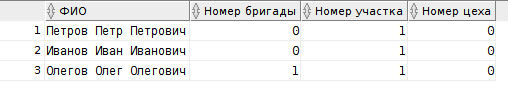
\includegraphics[width=11cm]{./screenshots/results/result6.png}

    \item Перечень мастеров (ФИО) указанного участка указанного цеха и номера бригад, работы которых они координируют.

    \lstinputlisting[language=SQL]{../sources/queries/task7.sql}

    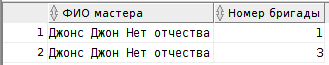
\includegraphics[width=11cm]{./screenshots/results/result7.png}

    \item Информация о цехах, в которых в настоящий момент собирается больше видов изделий, чем в среднем приходится на каждый производственный цех предприятия: номер цеха, название цеха, кол-во собираемых видов изделий, среднее количество видов изделий по цехам предприятия.

    \lstinputlisting[language=SQL]{../sources/queries/task8.sql}

    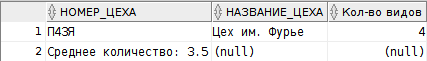
\includegraphics[width=11cm]{./screenshots/results/result8.png}

    \item Состав бригад, участвующих в сборке указанной категории изделия.

    \lstinputlisting[language=SQL]{../sources/queries/task9.sql}

    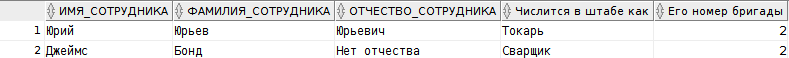
\includegraphics[width=11cm]{./screenshots/results/result9.png}

    \item ФИО и должности работников цеха, в котором собирается больше всего категорий изделий.

    \lstinputlisting[language=SQL]{../sources/queries/task10.sql}

    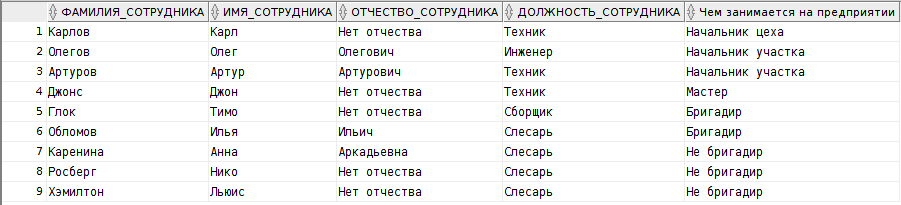
\includegraphics[width=11cm]{./screenshots/results/result10.png}

\end{enumerate}

\section{Создание представления}
Создал view представление запроса №4.
Так как все запросы, кроме 4, 8 и 10 нуждаются в подстановочных переменных.
10 запрос требует операции со множествами (именно UNION), а 8 LEFT JOIN.
Следовательно, был выбран единственный вариант, именно 4 запрос.
Однако с небольшим изменением, так как в 4 запросе использован UNION ALL, чтобы аккуратно добавить его в конец таблицы.
А в представлении это же значение удалось вывести в последнюю колонку.

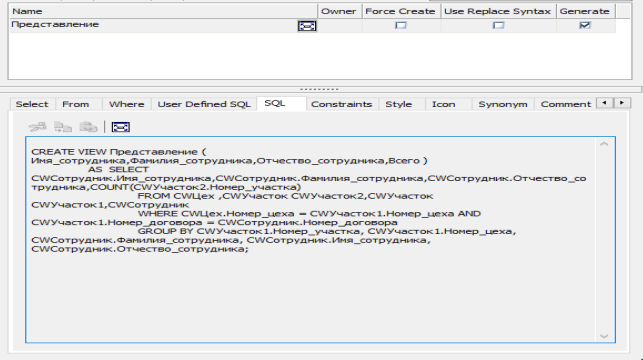
\includegraphics[width=11cm]{./screenshots/view/sql.png}

Результат удовлетворяет требованиям и схож с запросом.

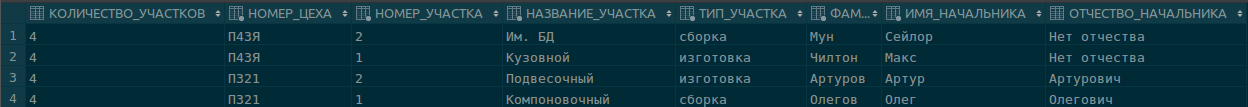
\includegraphics[width=11cm]{./screenshots/view/result.png}

\section{Доказательства выполнения ограничивающих требований, привиденных в описании предметной области}

Проведем проверку.

Попробуем добавить уже существую категорию:

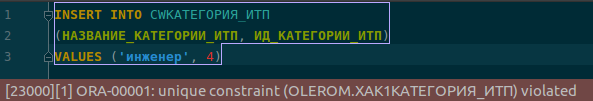
\includegraphics[width=11cm]{./screenshots/constraints/cat_itp.png}

Попробуем добавить участок, с неправильным типом:

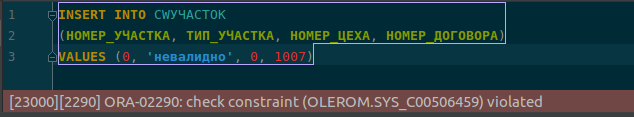
\includegraphics[width=11cm]{./screenshots/constraints/field_type.png}

Попробуем добавить участок, с несуществующим руководителем:

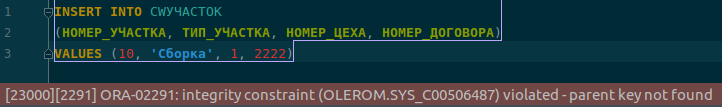
\includegraphics[width=11cm]{./screenshots/constraints/field.png}

Попробуем добавить запись в журнал для несуществующего вида:

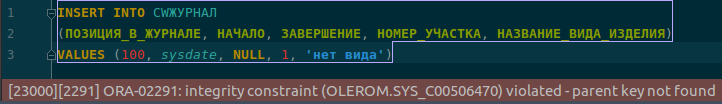
\includegraphics[width=11cm]{./screenshots/constraints/list.png}

Попробуем добавить запись в журнал для несуществующего вида:

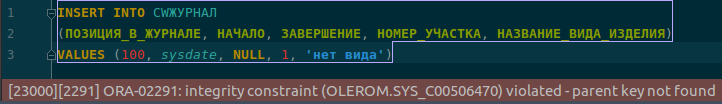
\includegraphics[width=11cm]{./screenshots/constraints/list.png}

\section{Приложение 1}

    Логическая модель.

    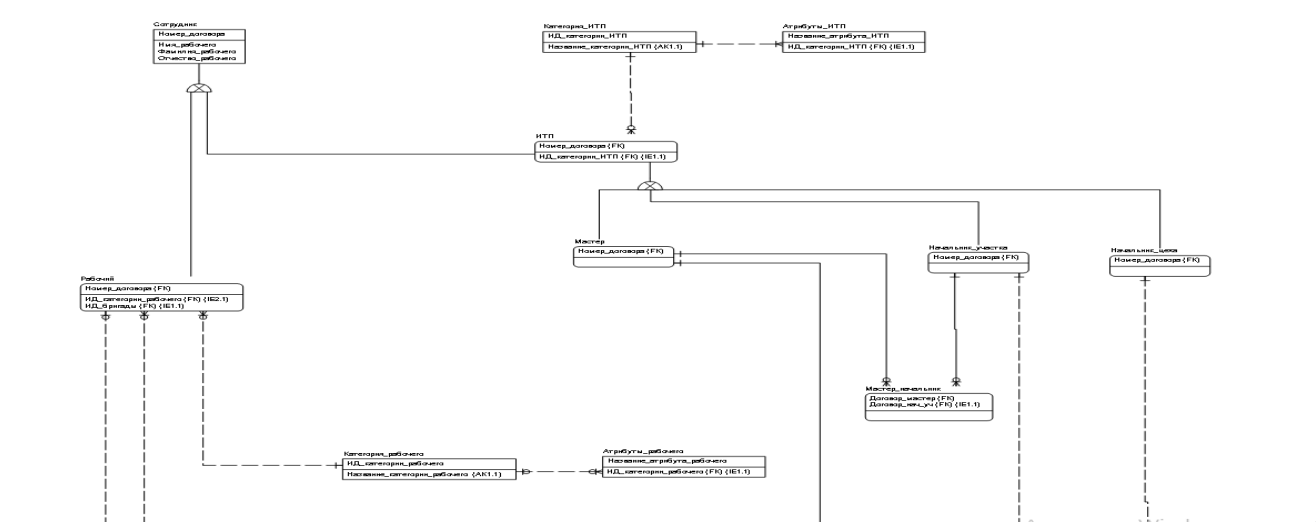
\includegraphics[width=11cm]{./screenshots/model/logical1.png}

    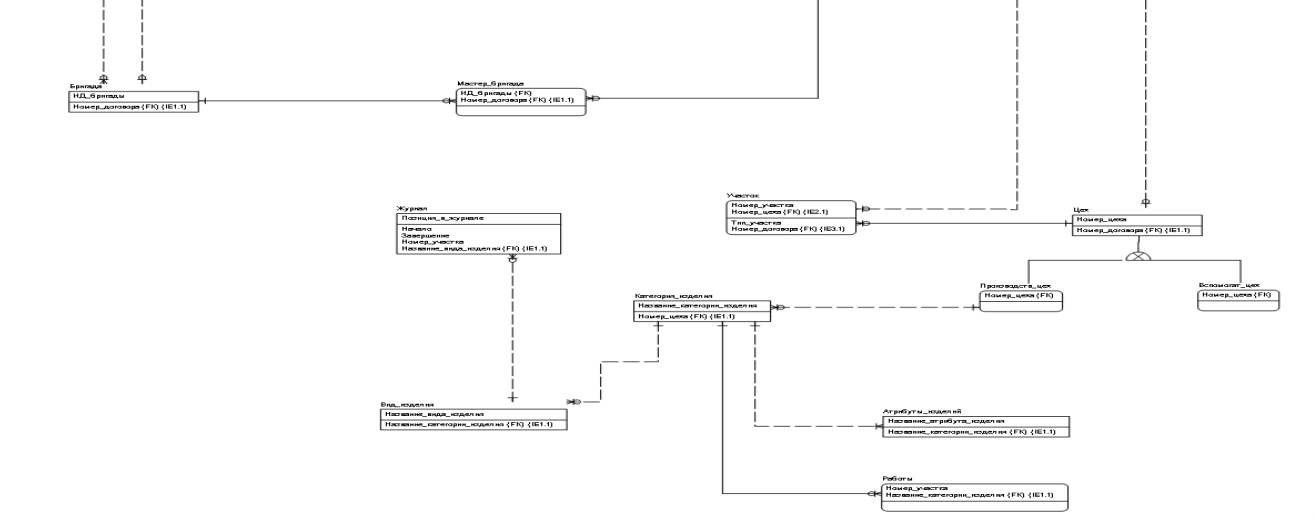
\includegraphics[width=11cm]{./screenshots/model/logical2.png}

\section{Приложение 2}

    Физическая модель.

    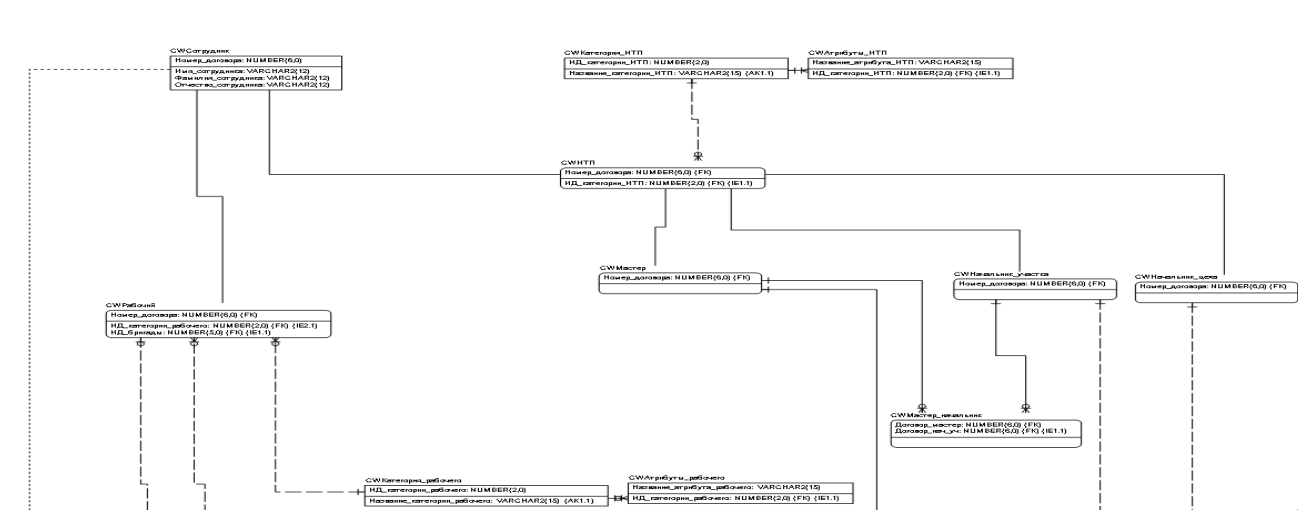
\includegraphics[width=11cm]{./screenshots/model/physical1.png}

    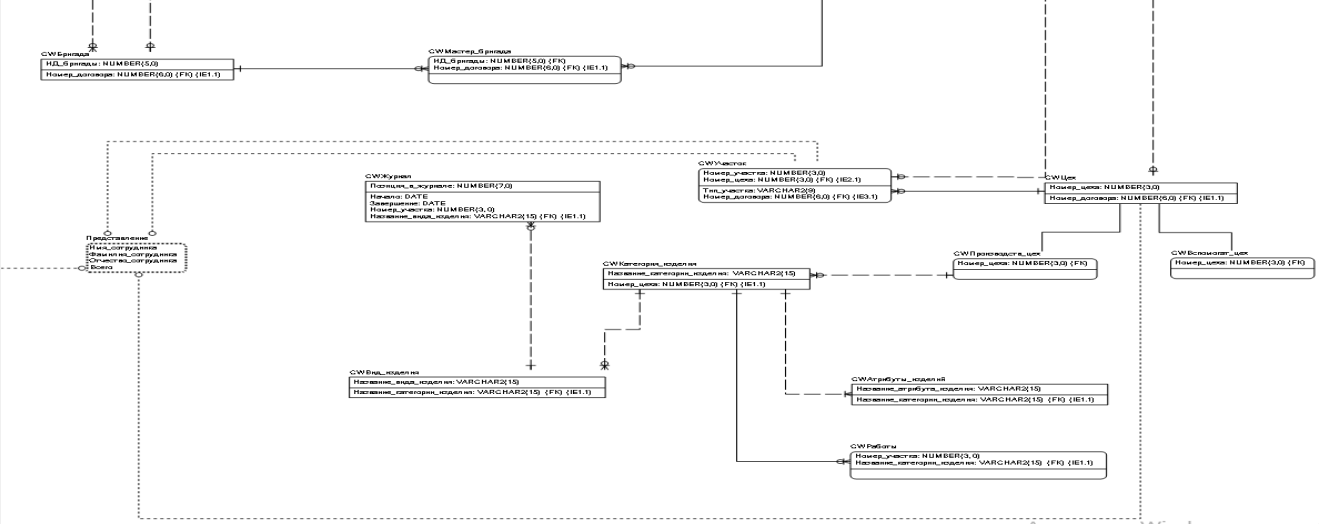
\includegraphics[width=11cm]{./screenshots/model/physical2.png}

\section{Приложение 3}

    Физическая модель после обратного проектирования.

    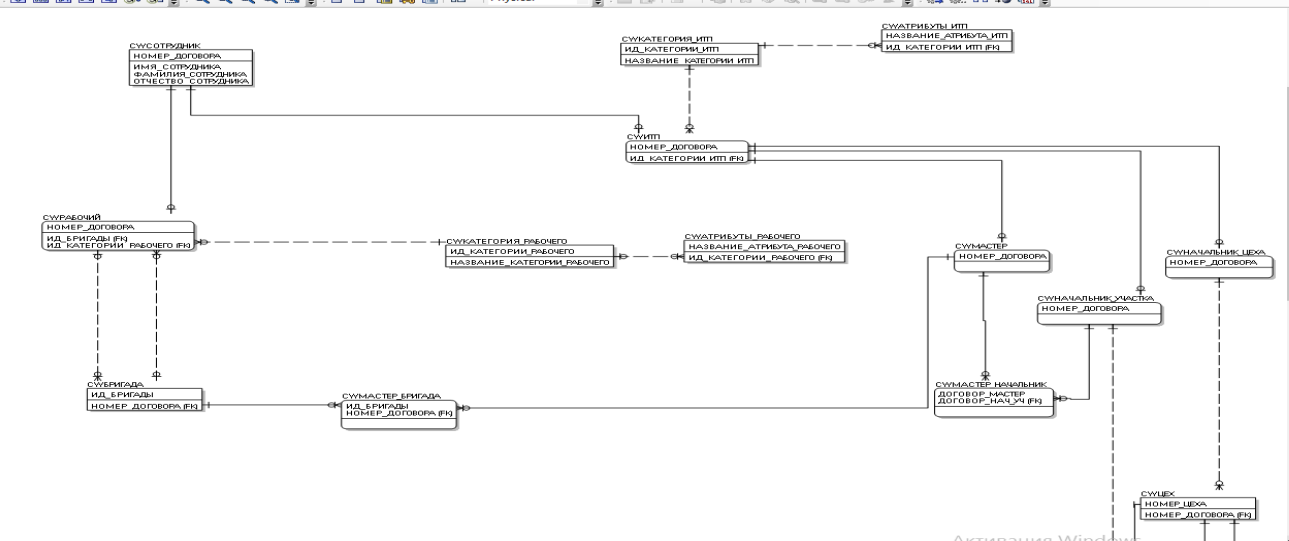
\includegraphics[width=11cm]{./screenshots/model/reverse1.png}

    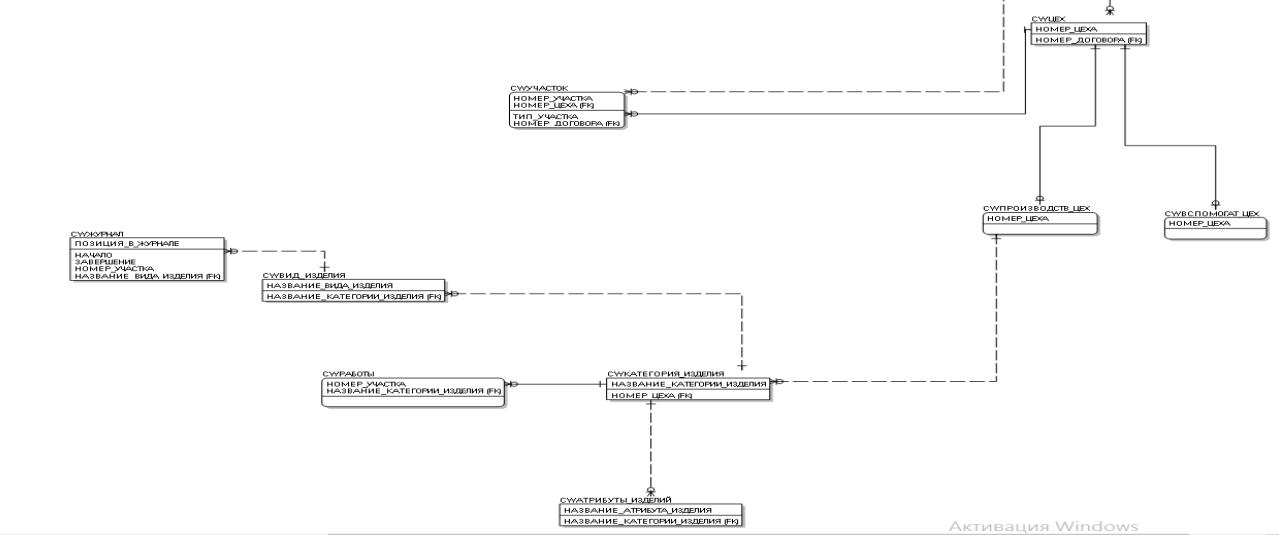
\includegraphics[width=11cm]{./screenshots/model/reverse2.png}

\section{Заключение}
В результате работы была спроектирована информационная система автомобилестроительного предприятия.
Была проведена нормализация разработанной модели до 5НФ.
Была проверена разработанная модель мредствами ERwin Data Model Validator r7, а также устранены все возможные замечания.
Проведено прямое и обратное проектирование.
Создано представление на основе 4 запроса.
Созданы 10 SQL-запросов и проверена их работоспособность.

Были закреплены теоретические и пркатические знания.

\section{Список использованных источников}

\begin{enumerate}

    \item Конспект лекций
    \item БАЗЫ ДАННЫХ. ПРАКТИКУМ. ЧАСТЬ 2. ORACLE SQL, О. Ю. Сабинин, Н. В. Андреева
    \item Материалы, доступные на dl.spbstu.ru

\end{enumerate}

\end{document}